\documentclass[tikz]{standalone}
\usepackage[T1]{fontenc}
\usepackage{newtxtext}
\usepackage[smallerops]{newtxmath}
\usepackage{varwidth}
\usepackage{xcolor}
\usetikzlibrary{positioning}
\tikzset{
    cnode/.style = {circle, draw=blue!50, fill=blue!20, minimum size=2.5em}
    hidden/.style = {opacity = 0.3}
}

\begin{document}
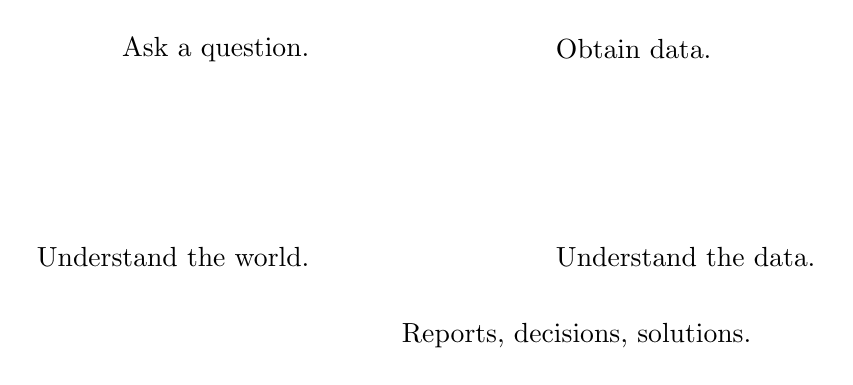
\begin{tikzpicture}[align=center, node distance=7.5em]
\node[cnode, label=left:Ask a question.] (ask) {};
\node[cnode, label=right:Obtain data., right of=ask] (data) {};
\node[cnode, label=left:Understand the world., below of=ask] (uworld) {};
\node[cnode, label=right:Understand the data., right of=uworld] (udata) {};
\coordinate[above=2.5em of ask] (aup);
\coordinate[above=2.5em of data] (dup);
\coordinate[label={[xshift=-2mm]right:Reports, decisions, solutions.}, below right=2.5em and 2.5em of uworld] {};
\
% \draw [->, line width=0.25mm] (edge (ask) (dup) edge (data) (ask) edge (data) (data) edge (udata) (udata) edge (uworld) (uworld) edge (ask) (udata) edge (ask);
% \draw [->, bend right, line width=0.25mm] (udata) edge (data);
% \draw [->, to path = (\tikztostart) |- (\tikztotarget), line width=0.25mm] (uworld) edge (result);
\end{tikzpicture}
\end{document}
